%!TEX root = ./Structure_rapport_final.tex


Resitue le sujet dans une problématique générale ;
 -restitue le sujet dans un cadre de gestion plus global
- doit également justifier le bien-fondé de l’étude en fonction des demandes
• Donne les objectifs qui ont été fixés pour répondre à la question posée ;
• Présente la démarche qui va permettre de répondre aux objectifs.


\subsection{Présentation des milieux marins profonds}
- milieu peu connu, écosystème particulier --> communauté sur laquelle on travaille 
- particuliarité des canyons 
- Rôle de ces espèces dans les chaines trophiques (plus faibles maillons et MM/oiseaux)
- communauté de poisson méso-bathy pélagiques 


Deep-sea is the largest marine habitat of Earth, and represents 95\% of ocean's volume \citep{danovaro2017,salazar2016}. From a biology perspective, deep-sea encompasses everything underneath euphotic (or epipelagial) zone, where the solar radiations are too low and precludes photosynthesis \citep{baker2020,danovaro2017,salazar2016} (see Figure~\ref{fig:dsl}). Between 200 to 1000m deep (mesopelagic zone), light fades and temperature decreases, because solar luminance is absorbed exponentially in upper sea layers \citep{reynolds2001}. After 1000m deep (bathypelagic zone), no sunlight remains and the habitat is pitch-black; salinity and temperature are stable (between -1.8 to 2°C), and pressure keeps on increasing by 1 atm every 10m. 

\begin{figure} [!htbp]
	\begin{center}
		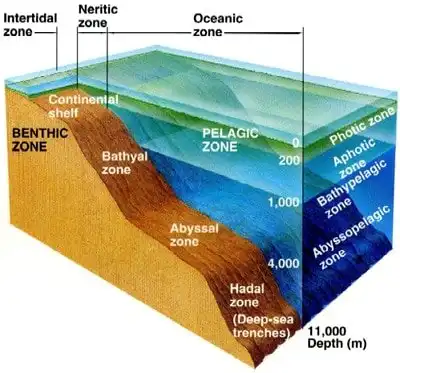
\includegraphics[width=0.8\textwidth]{sea_layers.png}
	\end{center}
	\caption[Petite légende]{Sea layers along depth, from \citep{fig_deep_sea}}
	\label{fig:dsl}
\end{figure}

Despite those extremes conditions, and low rate of food supply deep-sea is far from being lifeless. In fact, deep-sea is considered to be the largest biome of the Earth, and contains 70\% of ocean's microbial cells and 60\% of its heterotrophic activity, playing a crucial role in biogeochemical cycles \citep{salazar2016}. \citet{grassle1992,parkes1994,todo2005} studies shown that life could be found everywhere in the deep-sea, with remarkably high and stable diversity. With first studies launched in the 60's, less that 0.0001\% of the area has been investigated so far \citep{danovaro2017}. Thus, deep-sea remains the most unknown biome of the planet with estimated 10 million species that are yet to discover \citep{danovaro2017,grassle1992}. In particular, data are lacking to evaluate the impact of climate change on the biodiversity of the largest reservoir of biomass, mainly because exploring deep-sea is difficult and requires specific tools, such as rovers \citep{danovaro2008,danovaro2014}. Firstly, deep-sea were regarded as a ore reservoir, where manganese and other metal deposits could be found and extracted, or even as a dumping site for nuclear wastes \citep{baker2020,gillet2013,halfar2002}. But since past decades, capacity of exploration of the deep-sea expanded spectacularly, allowing seachers to discover more about the depth of the oceans \citep{danovaro2014}.
In particular, continental margins, which separates continental shelf from abyssal plains are investigated, because their heterogeneous topography implies varied habitats and hydrodynamics, with impacts on the whole food chain \citep{danovaro2009}. Along continental margins, deep-sea canyons, that incises the edges of continental shelf, appears to be ``biodiversity hotspots'' for pelagic life, in terms of diversity and abundance \citep{aissi2012,danovaro2009,gillet2013,robertson2020}. Because they are the main conduits transfering organic matter and sediments from rich and productive shallow shelf to the low-nutrients deep-sea, canyons constitues peculiar habitats, with evidences of an important biomass and diversity of benthic organisms \citep{canals2006,danovaro2009,leo2012}, but also of fishes assemblages \citep{sion2019,stefanescu1994}. Locally, canyons displays higher nutrients concentrations than in adjacent areas, due to down-welling currents, that makes them favourable habitats for filters and suspension feeders \citep{sion2019}. Abundance of nutrients and preys attracts top predators, some of them being only encountered in those habitats \citep{aissi2012}. Among abundant preys are found euphausiids, shrimps, squids and meso- and bathypelagic fishes \citep{aissi2012,gaskett2001}.

Meso- and bathypelagic fishes are found in every ocean, except Arctic, and are the dominant zooplankton consumers in most oceans, playing a key role in trophic networks \citep{davison2015}~. Living between 200-1000m (mesopelagic) and over 1000m (bathypelagic) deep, those fishes displays very high biomass, mainly carried by Myctophidae family \citep{gaskett2001,kozlov1995,pusch2004}. 

Therefore, 







\subsection{Axes pour une meilleure connaissance de ces écosystèmes}
- comment les espèces se partagent les ressources (bcp d'études déjà terrestres)
         --> focus sur cette communauté particulière qui est pour l'instant peu connue

- 2 approches possibles: 
		- espèce-centrée : seule ou en compétition --> mais limitant pour la comparaison entre écosystèmes différents. 
		- communautaire : certaines espèces sont-elles redondantes ? Plusieurs espèces
occupent la même niche en cas de chevauchement, occupent la même niche fonctionnelle. Se focaliser
sur les fonctions plutôt que sur l'espèce. --> Permet une généralisation de la méthode et une comparaison entre écosystèmes
		- Individus appartenant à la meme niche peuvent être considérés comme appartenant
à la même boîte fonctionelle. 
==> Caractériser un écosystème par les fonctions qu'ils présentent plutôt que par ses espèces

\subsection{Présentation de la démarche et des objectifs}
- mieux connaitre ces communautés à travers les niches qu'elles occupent dans les écosystèmes
- caractériser leurs niches trophiques, comportements, habitats, sensibilité des espèces, 
particularité des espèces, voir les avantages de partager les niches 
- Envisager une approche universelle, permettant la comparaison d'écosystèmes

- Hypothèses: chevauchement de niches entre les espèces, entrainant de la compétition entre les espèces ayant des fonctions similaires, ou ségrégation, où les espèces
utilisent des ressources distinctes et ont des fonctions différentes

